
%{{第三十一回}}{第三十一回}}

\chapter{撕扇子作千金一笑 因麒麟伏白首双星}\label{part0035_split_000.htmlux5cux23calibre_pb_0}

{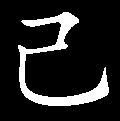
\includegraphics[width=3mm]{../Images/00003}``撕扇子''是以不知情之物,供娇嗔不知情事之人一笑,所谓``情不情''。}

{``金玉姻缘''已定,又写一金麒麟,是间色法也。何颦儿为其所惑?故颦儿谓``情情''。}

话说袭人见了自己吐的鲜血在地,也就冷了半截,想着往日常听人说:``少年吐血,年月不保,纵然命长,终是废人了。''想起此言,不觉将素日想着后来争荣夸耀之心尽皆灰了,眼中不觉滴下泪来。宝玉见他哭了,也不觉心酸起来,因问道:``你心里觉的怎么样?''袭人勉强笑道:``好好的,觉怎么呢。''宝玉的意思即刻便要叫人烫黄酒,要山羊血黎洞丸来。袭人拉了他的手,笑道:``你这一闹不打紧,闹起多少人来,倒抱怨我轻狂。分明人不知道,倒闹的人知道了,你也不好,我也不好。正经明儿你打发小子问问王太医去,弄点子药吃吃就好了。人不知鬼不觉的可不好?''宝玉听了有理,也只得罢了,向案上斟了茶来,给袭人漱了口。袭人知宝玉心内是不安稳的,待要不叫他伏侍,他又必不依;二则定要惊动别人,不如由他去罢:因此只在榻上由宝玉去伏侍。

一交五更,宝玉也顾不的梳洗,忙穿衣出来,将王济仁叫来,亲自确问。王济仁问其原故,不过是伤损,便说了个丸药的名字,怎么服,怎么敷。宝玉记了,回园依方调治。不在话下。

这日正是端阳佳节,蒲艾簪门,虎符系臂。午间,王夫人治了酒席,请薛家母女等赏午。宝玉见宝钗淡淡的,也不和他说话,自知是昨儿的原故。王夫人见宝玉没精打彩,也只当是金钏儿昨日之事,他没好意思的,越发不理他。林黛玉见宝玉懒懒的,只当是他因为得罪了宝钗的原故,心中不自在,形容也就懒懒的。凤姐昨日晚间王夫人就告诉了他宝玉金钏的事,知道
王夫人不自在,自己如何敢说笑,也就随着王夫人的气色行事,更觉淡淡的。贾迎春姊妹见众人无意思,也都无意思了。因此,大家坐了一坐就散了。

林黛玉天性喜散不喜聚。他想的也有个道理,他说,``人有聚就有散,聚时欢喜,到散时岂不清冷?既清冷则生伤感,所以不如倒是不聚的好。比如那花开时令人爱慕,谢时则增惆怅,所以倒是不开的好。''故此人以为喜之时,他反以为悲。那宝玉的情性只愿常聚,生怕一时散了添悲;那花只愿常开,生怕一时谢了没趣;只到筵散花谢,虽有万种悲伤,也就无可如何了。

因此,今日之筵,大家无兴散了,林黛玉倒不觉得,倒是宝玉心中闷闷不乐,回至自己房中长吁短叹。偏生晴雯上来换衣服,不防又把扇子失了手跌在地下,将股子跌折。宝玉因叹道:``蠢才,蠢才!将来怎么样?明日你自己当家立事,难道也是这么顾前不顾后的?''晴雯冷笑道:``二爷近来气大的很,行动就给脸子瞧。前儿连袭人都打了,今儿又来寻我们的不是。要踢要打凭爷去。就是跌了扇子,也是平常的事。先时连那么样的玻璃缸、玛瑙碗不知弄坏了多少,也没见个大气儿,这会子一把扇子就这么着了。何苦来!要嫌我们就打发我们,再挑好的使。好离好散的,倒不好?''宝玉听了这些话,气的浑身乱战,因说道:``你不用忙,将来有散的日子!''

袭人在那边早已听见,忙赶过来向宝玉道:``好好的,又怎么了?可是我说的:`一时我不到,就有事故儿。'''晴雯听了冷笑道:``姐姐既会说,就该早来,也省了爷生气。自古以来,就是你一个人伏侍爷的,我们原没伏侍过。因为你伏侍的好,昨日才挨窝心脚;我们不会伏侍的,到明儿还不知是个什么罪呢!''袭人听了这话,又是恼,又是愧,待要说几句话,又见宝玉已经气的黄了脸,少不得自己忍了性子,推晴雯道:``好妹妹,你出去逛逛,原是我们的不是。''

晴雯听他说``我们''两个字,自然是他和宝玉了,不觉又添了酸意,冷笑几声,道:``我倒不知道你们是谁,别教我替你们害臊了!便是你们鬼鬼祟祟干的那事儿,也瞒不过我去,那里就称起`我们'来了。明公正道,连个姑娘还没挣上去呢,也不过和我似的,那里就称上`我们'了!''袭人羞的脸紫胀起来,想一想,原来是自己把话说错了。宝玉一面说:``你们气不忿,我明儿偏抬举他。''袭人忙拉了宝玉的手道:``他一个糊涂人,你和他分证什么?况且你素日又是有担待的,比这大的过去了多少,今儿是怎么了?''晴雯冷笑道:``我原是糊涂人,那里配和我说话呢!''袭人听说道:``姑娘倒是和我拌嘴呢,是和二爷拌嘴呢?要是心里恼我,你只和我说,不犯着当着二爷吵;要是恼二爷,不该这么吵的万人知道。我才也不过为了事,进来劝开了,大家保重。姑娘倒寻上我的晦气。又不像是恼我,又不像是恼二爷,夹枪带棒,终久是个什么主意?我就不多说,让你说去。''说着便往外走。

宝玉向晴雯道:``你也不用生气,我也猜着你的心事了。我回太太去,你也大了,打发你出去好不好?''晴雯听了这话,不觉又伤起心来,含恨说道:``为什么我出去?要嫌我,变着法儿打发我出去,也不能够。''宝玉道:``我何曾经过这个吵闹?一定是你要出去了。不如回太太,打发你去吧。''说着,站起来就要走。袭人忙回身拦住,笑道:``往那里去?''宝玉道:``回太太去。''袭人笑道:``好没意思!真个的去回,你也不怕臊了?便是他认真的要去,也等把这气下去了,等无事中说话儿回了太太也不迟。这会子急急的当作一件正经事去回,岂不叫太太犯疑?''宝玉道:``太太必不犯疑,我只明说是他闹着要去的。''晴雯哭道:``我多早晚闹着要去了?饶生了气,还拿话压派我。只管去回,我一头碰死了也不出这门儿。''宝玉道:``这也奇了。你又不去,你又闹些什么?我经不起这吵,不如去了倒干净。''说着一定要去回。袭人见拦不住,只得跪下了。碧痕、秋纹、麝月等众丫鬟见吵闹,都鸦雀无闻的在外头听消息,这会子听见袭人跪下央求,便一齐进来都跪下了。宝玉忙把袭人扶起来,叹了一声,在床上坐下,叫众人起去,向袭人道:``叫我怎么样才好!这个心使碎了也没人知道。''说着不觉滴下泪来。袭人见宝玉流下泪来,自己也就哭了。

晴雯在旁哭着,方欲说话,只见林黛玉进来,便出去了。林黛玉笑道:``大节下怎么好好的哭起来?难道是为争粽子吃争恼了不成?''宝玉和袭人``嗤''的一笑。黛玉道:``二哥哥不告诉我,我问你就知道了。''一面说,一面拍着袭人的肩,笑道:``好嫂子,你告诉我。必定是你两个拌了嘴了。告诉妹妹,替你们和劝和劝。''袭人推他道:``林姑娘你闹什么?我们一个丫头,姑娘只是混说。''黛玉笑道:``你说你是丫头,我只拿你当嫂子待。''宝玉道:``你何苦来替他招骂名儿。饶这么着,还有人说闲话,还搁的住你来说他。''袭人笑道:``林姑娘,你不知道我的心事,除非一口气不来死了倒也罢了。''林黛玉笑道:``你死了,别人不知怎么样,我先就哭死了。''宝玉笑道:``你死了,我作和尚去。''袭人笑道:``你老实些罢,何苦还说这些话。''林黛玉将两个指头一伸,抿嘴笑道:``作了两个和尚了。我从今以后都记着你作和尚的遭数儿。''宝玉听得,知道是他点前儿的话,自己一笑也就罢了。

一时黛玉去后,就有人说``薛大爷请'',宝玉只得去了。原来是吃酒,不能推辞,只得尽席而散。

晚间回来,已带了几分酒,踉跄来至自己院内,只见院中早把乘凉枕榻设下,榻上有个人睡着。宝玉只当是袭人,一面在榻沿上坐下,一面推他,问道:``疼的好些了?''只见那人翻身起来说:``何苦来,又招我!''宝玉一看,原来不是袭人,却是晴雯。宝玉将他一拉,拉在身旁坐下,笑道:``你的性子越发惯娇了。早起就是跌了扇子,我不过说了那两句,你就说上那些话。说我也罢了,袭人好意来劝,你又括上他,你自己想想,该不该?''晴雯道:``怪热的,拉拉扯扯作什么!叫人来看见像什么!我这身子也不配坐在这里。''宝玉笑道:``你既知道不配,为什么睡着呢?''晴雯没的话,``嗤''的又笑了,说:``你不来便使得,你来了就不配了。起来,让我洗澡去。袭人麝月都洗了澡,我叫了他们来。''宝玉笑道:``我才又吃了好些酒,还得洗一洗。你既没有洗,拿了水来咱们两个洗。''

晴雯摇手笑道:``罢,罢,我不敢惹爷。还记得碧痕打发你洗澡,足有两三个时辰,也不知道作什么呢。我们也不好进去的。后来洗完了,进去瞧瞧,地下的水淹着床腿,连席子上都汪着水,也不知是怎么洗了,笑了几天。我也没那工夫收拾,也不用同我洗去。今儿也凉快,那会子洗了,可以不用再洗。我倒舀一盆水来,你洗洗脸通通头。才刚鸳鸯送了好些果子来,都湃在那水晶缸里呢,叫他们打发你吃。''宝玉笑道:``既这么着,你也不许洗去,只洗洗手来拿果子来吃罢。''晴雯笑道:``我慌张的很,连扇子还跌折了,那里还配打发吃果子。倘或再打破了盘子,还更了不得呢。''宝玉笑道:``你爱打就打,这些东西原不过是借人所用,你爱这样,我爱那样,各自性情不同。比如那扇子原是扇的,你要撕着玩也可以使得,只是不可生气时拿他出气。就如杯盘,原是盛东西的,你喜听那一声响,就故意的碎了也可以使得,只是别在生气时拿他出气。这就是爱物了。''晴雯听了,笑道:``既这么说,你就拿了扇子来我撕。我最喜欢撕的。''宝玉听了,便笑着递与他。晴雯果然接过来,``嗤''的一声,撕了两半,接着``嗤嗤''又听几声。宝玉在旁笑着说:``响的好,再撕响些!''

正说着,只见麝月走过来,笑道:``少作些孽罢。''宝玉赶上来,一把将他手里的扇子也夺了递与晴雯。晴雯接了,也撕了几半子,二人都大笑。麝月道:``这是怎么说,拿我的东西开心儿?''宝玉笑道:``打开扇子匣子你拣去,什么好东西!''麝月道:``既这么说,就把匣子搬了出来,让他尽力的撕,岂不好?''宝玉笑道:``你就搬去。''麝月道:``我可不造这孽。他也没折了手,叫他自己搬去。''晴雯笑着,倚在床上说道:``我也乏了,明儿再撕罢。''宝玉笑道:``古人云:`千金难买一笑。'几把扇子能值几何!''一面说着,一面叫袭人。袭人才换了衣服走出来,小丫头佳蕙过来拾去破扇,大家乘凉,不消细说。

至次日午间,王夫人、薛宝钗、林黛玉众姊妹正在贾母房内坐着,就有人回:``史大姑娘来了。''一时果见史湘云带领众多丫鬟媳妇走进院来。宝钗黛玉等忙迎至阶下相见。青年姊妹间经月不见,一旦相逢,其亲密自不必细说。

一时进入房中,请安问好,都见过了。贾母因说:``天热,把外头的衣服脱脱罢。''史湘云忙起身宽衣。王夫人因笑道:``也没见穿上这些作什么?''史湘云笑道:``都是二婶婶叫穿的,谁愿意穿这些。''宝钗一旁笑道:``姨娘不知道,他穿衣裳还更爱穿别人的衣裳。可记得旧年三四月里,他在这里住着,把宝兄弟的袍子穿上,靴子也穿上,额子也勒上,猛一瞧倒像是宝兄弟,就是多两个坠子。他站在那椅子后边,哄的老太太只是叫`宝玉,你过来,仔细那上头挂的灯穗子招下灰来迷了眼'。他只是笑,也不过去。后来大家撑不住笑了,老太太才笑了,说:`倒扮上男人好看了。'''林黛玉道:``这算什么。惟有前年正月里接了他来,住了没两日就下起雪来,老太太和舅母那日想是才拜了影回来,老太太的一个新新的大红猩猩毡斗蓬放在那里,谁知眼错不见他就披了,又大又长,他就拿了个汗巾子拦腰系上,和丫头们在后院子扑雪人儿去,一跤栽到沟跟前,弄了一身泥水。''说着,大家想着前情,都笑了。

宝钗笑向那周奶妈道:``周妈,你们姑娘还是那么淘气不淘气了?''周奶娘也笑了。迎春笑道:``淘气也罢了,我就嫌他爱说话。也没见睡在那里还是咭咭呱呱,笑一阵,说一阵,也不知那里来的那些话。''王夫人道:``只怕如今好了。前日有人家来相看,眼见有婆婆家了,还是那么着。''贾母因问:``今儿还是住着,还是家去呢?''周奶娘笑道:``老太太没有看见衣服都带了来,可不住两天?''史湘云问道:``宝玉哥哥不在家么?''宝钗笑道:``他再不想着别人,只想宝兄弟,两个人好憨的。这可见还没改了淘气。''贾母道:``如今你们大了,别提小名儿了。''

刚只说着,只见宝玉来了,笑道:``云妹妹来了。怎么前儿打发人接你去,怎么不来?''王夫人道:``这里老太太才说这一个,他又来提名道姓的了。''林黛玉道:``你哥哥得了好东西,等着你呢。''史湘云道:``什么好东西?''宝玉笑道:``你信他呢!几日不见,越发高了。''湘云笑道:``袭人姐姐好?''宝玉道:``多谢你记挂。''湘云道:``我给他带了好东西来了。''说着,拿出手帕子来,挽着一个疙瘩。宝玉道:``什么好的?你倒不如把前儿送来的那种绛纹石的戒指儿带两个给他。''湘云笑道:``这是什么?''说着便打开。众人看时,果然就是上次送来的那绛纹戒指,一包四个。林黛玉笑道:``你们瞧瞧他这主意。前儿一般的打发人给我们送了来,你就把他的带来岂不省事?今儿巴巴的自己带了来,我当又是什么新奇东西,原来还是他。真真你是糊涂人。''史湘云笑道:``你才糊涂呢!我把这理说出来,大家评一评谁糊涂。给你们送东西,就是使来的不用说话,拿进来一看,自然就知是送姑娘们的了;若带他们的东西,这得我先告诉来人,这是那一个丫头的,那是那一个丫头的,那使来的人明白还好,再糊涂些,丫头的名字他也不记得,混闹胡说的,反连你们的东西都搅糊涂了。若是打发个女人素日知道的还罢了,偏生前儿又打发小子来,可怎么说丫头们的名字呢?横竖我来给他们带来,岂不清白。''说着,把四个戒指放下,说道:``袭人姐姐一个,鸳鸯姐姐一个,金钏儿姐姐一个,平儿姐姐一个:这倒是四个人的,难道小子们也记得这么清白?''众人听了都笑道:``果然明白。''宝玉笑道:``还是这么会说话,不让人。''林黛玉听了,冷笑道:``他不会说话,他的金麒麟会说话。''一面说着,便起身走了。幸而诸人都不曾听见,只有薛宝钗抿嘴一笑。宝玉听见了,倒自己后悔又说错了话,忽见宝钗一笑,由不得也笑了。宝钗见宝玉笑了,忙起身走开,找了林黛玉去说话。

贾母向湘云道:``吃了茶歇一歇,瞧瞧你的嫂子们去。园里也凉快,同你姐姐们去逛逛。''湘云答应了,将三个戒指儿包上,歇了一歇,便起身要瞧凤姐等人去。众奶娘丫头跟着,到了凤姐那里,说笑了一回,出来便往大观园来,见过了李宫裁,少坐片时,便往怡红院来找袭人。因回头说道:``你们不必跟着,只管瞧你们的朋友亲戚去,留下翠缕伏侍就是了。''众人听了,自去寻姑觅嫂,早剩下湘云翠缕两个人。

翠缕道:``这荷花怎么还不开?''史湘云道:``时候没到。''翠缕道:``这也和咱们家池子里的一样,也是楼子花?''湘云道:``他们这个还不如咱们的。''翠缕道:``他们那边有棵石榴,接连四五枝,真是楼子上起楼子,这也难为他长。''史湘云道:``花草也是同人一样,气脉充足,长的就好。''翠缕把脸一扭,说道:``我不信这话。若说同人一样,我怎么不见头上又长出一个头来的人?''湘云听了由不得一笑,说道:``我说你不用说话,你偏好说。这叫人怎么好答言?天地间都赋阴阳二气所生,或正或邪,或奇或怪,千变万化,都是阴阳顺逆多少,一生出来,人罕见的就奇,究竟理还是一样。''翠缕道:``这么说起来,从古至今,开天辟地,都是阴阳了?''湘云笑道:``糊涂东西,越说越放屁。什么`都是些阴阳',难道还有个`阴阳'不成!`阴'`阳'两个字还只是一字,阳尽了就成阴,阴尽了就成阳,不是阴尽了又有个阳生出来,阳尽了又有个阴生出来。''翠缕道:``这糊涂死了我!什么是个阴阳,没影没形的。我只问姑娘,这阴阳是怎么个样儿?''湘云道:``阴阳可有什么样儿,不过是个气,器物赋了成形。比如天是阳,地就是阴;水是阴,火就是阳;日是阳,月就是阴。''

翠缕听了,笑道:``是了,是了,我今儿可明白了。怪道人都管着日头叫`太阳'呢,算命的管着月亮叫什么`太阴星',就是这个理了。''湘云笑道:``阿弥陀佛!刚刚的明白了。''翠缕道:``这些大东西有阴阳也罢了,难道那些蚊子、虼蚤、蠓虫儿、花儿、草儿、瓦片儿、砖头儿也有阴阳不成?''湘云道:``怎么有没阴阳的呢?比如那一个树叶儿还分阴阳呢,那边向上朝阳的便是阳,这边背阴覆下的便是阴。''翠缕听了,点头笑道:``原来这样,我可明白了。只是咱们这手里的扇子,怎么是阳,怎么是阴呢?''湘云道:``这边正面就是阳,那边反面就为阴。''翠缕又点头笑了,还要拿几件东西问,因想不起个什么来,猛低头就看见湘云宫绦上系的金麒麟,便提起来问道:``姑娘,这个难道也有阴阳?''湘云道:``走兽飞禽,雄为阳,雌为阴;牝为阴,牡为阳。怎么没有呢!''翠缕道:``这是公的,到底是母的呢?''湘云道:``这连我也不知道。''翠缕道:``这也罢了,怎么东西都有阴阳,咱们人倒没有阴阳呢?''湘云照脸啐了一口道:``下流东西,好生走罢!越问越问出好的来了!''翠缕笑道:``这有什么不告诉我的呢?我也知道了,不用难我。''湘云笑道:``你知道什么?''翠缕道:``姑娘是阳,我就是阴。''说着,湘云拿手帕子握着嘴,呵呵的笑起来。翠缕道:``说是了,就笑的这样了。''湘云道:``很是,很是。''翠缕道:``人规矩主子为阳,奴才为阴。我连这个大道理也不懂得?''湘云笑道:``你很懂得。''

一面说,一面走,刚到蔷薇架下,湘云道:``你瞧那是谁掉的首饰,金晃晃在那里。''翠缕听了,忙赶上拾在手里攥着,笑道:``可分出阴阳来了。''说着,先拿史湘云的麒麟瞧。湘云要他拣的瞧,翠缕只管不放手,笑道:``是件宝贝,姑娘瞧不得。这是从那里来的?好奇怪!我从来在这里没见有人有这个。''湘云笑道:``拿来我看。''翠缕将手一撒,笑道:``请看。''湘云举目一验,却是文彩辉煌的一个金麒麟,比自己佩的又大又有文彩。湘云伸手擎在掌上,只是默默不语,正自出神,忽见宝玉从那边来了,笑问道:``你两个在这日头底下作什么呢?怎么不找袭人去?''湘云连忙将那麒麟藏起道:``正要去呢。咱们一处走。''说着,大家进入怡红院来。

袭人正在阶下倚槛追风,忽见湘云来了,连忙迎下来,携手笑说一向久别情况。一时进来归坐,宝玉因笑道:``你该早来,我得了一件好东西,专等你呢。''说着,一面在身上摸掏,掏了半天,``呵呀''了一声,便问袭人``那个东西你收起来了么?''袭人道:``什么东西?''宝玉道:``前儿得的麒麟。''袭人道:``你天天带在身上的,怎么问我?''宝玉听了,将手一拍说道:``这可丢了,往那里找去!''就要起身自己寻去。湘云听了,方知是他遗落的,便笑问道:``你几时又有了麒麟了?''宝玉道:``前儿好容易得的呢,不知多早晚丢了,我也糊涂了。''湘云笑道:``幸而是顽的东西,还是这么慌张。''说着,将手一撒,``你瞧瞧,是这个不是?''宝玉一见,由不得欢喜非常,因说道\ldots{}\ldots{}不知是如何,且听下回分解。

{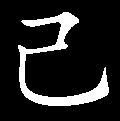
\includegraphics[width=3mm]{../Images/00003}后数十回若兰在射圃所佩之麒麟,正此麒麟也。提纲伏于此回中,所谓``草蛇灰线,在千里之外''。}
